\UseRawInputEncoding
    %%%%%%%%%%%%%%%%%%%%%%%%%%%%%%%%%%%%%%%%%
%  My documentation report
%  Objetive: Explain what I did and how, so someone can continue with the investigation
%
% Important note:
% Chapter heading images should have a 2:1 width:height ratio,
% e.g. 920px width and 460px height.
%
%%%%%%%%%%%%%%%%%%%%%%%%%%%%%%%%%%%%%%%%%


%----------------------------------------------------------------------------------------
%	PACKAGES AND OTHER DOCUMENT CONFIGURATIONS
%----------------------------------------------------------------------------------------

\documentclass[openany]{report} % Default font size and left-justified equations

\usepackage{minted}
\usemintedstyle{vim}
\usepackage{upquote}
\usepackage{textcomp}

\usepackage{enumitem}   % compact item/enum
\usepackage[breakable]{tcolorbox}  % shaded boxes with breakable option
\usepackage{booktabs}   % better tables
\usepackage{multirow}   % for multirow cells in tables
\usepackage{siunitx}    % \SI{15}{min}
\usepackage{listings}   % code blocks
\usepackage{float}      % for [H] figure placement

\usepackage[top=3cm,bottom=3cm,left=3.2cm,right=3.2cm,headsep=10pt,letterpaper]{geometry} % Page margins

\usepackage{xcolor} % Required for specifying colors by name
\definecolor{ocre}{RGB}{52,177,201} % Define the orange color used for highlighting throughout the book

% Font Settings
\usepackage{avant} % Use the Avantgarde font for headings
%\usepackage{times} % Use the Times font for headings
\usepackage{mathptmx} % Use the Adobe Times Roman as the default text font together with math symbols from the Sym­bol, Chancery and Com­puter Modern fonts
\usepackage{microtype} % Slightly tweak font spacing for aesthetics
\usepackage[utf8]{inputenc} % Required for including letters with accents
\usepackage[T1]{fontenc} % Use 8-bit encoding that has 256 glyphs
\usepackage{amsthm}
\usepackage{graphicx}
\usepackage{eso-pic}
\usepackage{xcolor}
\usepackage{fontenc} % Required for font selection
\usepackage{listings}
\usepackage{xcolor}
\usepackage{upquote}
\usepackage{textcomp}

\definecolor{codebg}{HTML}{F8F8F8}

\lstdefinestyle{bashstyle}{
  language=bash,
  basicstyle=\ttfamily\small,
  backgroundcolor=\color{codebg},
  columns=fullflexible,
  keepspaces=true,
  showstringspaces=false,
  frame=single,
  framerule=0.5pt,
  breaklines=true,
  postbreak=\mbox{\textcolor{gray}{$\hookrightarrow$}\space},
  keywordstyle=\color{blue},
  commentstyle=\color{gray},
  stringstyle=\color{orange},
  numbers=left,
  numberstyle=\tiny\color{gray},
  stepnumber=1,
  numbersep=10pt,
  tabsize=2
}

\usepackage{listings}
\usepackage{xcolor}
\usepackage{hyperref}

\definecolor{codebg}{HTML}{F8F8F8}
\lstset{
  backgroundcolor=\color{codebg},
  basicstyle=\ttfamily\small,
  columns=fullflexible,
  keepspaces=true,
  frame=single,
  breaklines=true,
  postbreak=\mbox{\textcolor{gray}{$\hookrightarrow$}\space}
}



% Bibliography
\usepackage[style=ieee,sorting=none,sortcites=true,autopunct=true,babel=hyphen,hyperref=true,abbreviate=false,backref=true,backend=bibtex]{biblatex}
\addbibresource{bibliography.bib} % BibTeX bibliography file
\defbibheading{bibempty}{}

\input{structure} % Insert the commands.tex file which contains the majority of the structure behind the template


\newcommand{\titlefont}[2]{{\fontsize{#1}{#1}\selectfont\textbf{#2}}}
\newcommand{\subtitlefont}[2]{{\fontsize{#1}{#1}\selectfont#2}}


%----------------------------------------------------------------------------------------
%	Definitions of new commands
%----------------------------------------------------------------------------------------

\def\R{\mathbb{R}}
\newcommand{\cvx}{convex}
\begin{document}

%----------------------------------------------------------------------------------------
%	TITLE PAGE
%----------------------------------------------------------------------------------------
\begingroup
\thispagestyle{empty}
\AddToShipoutPicture*{\put(0,0){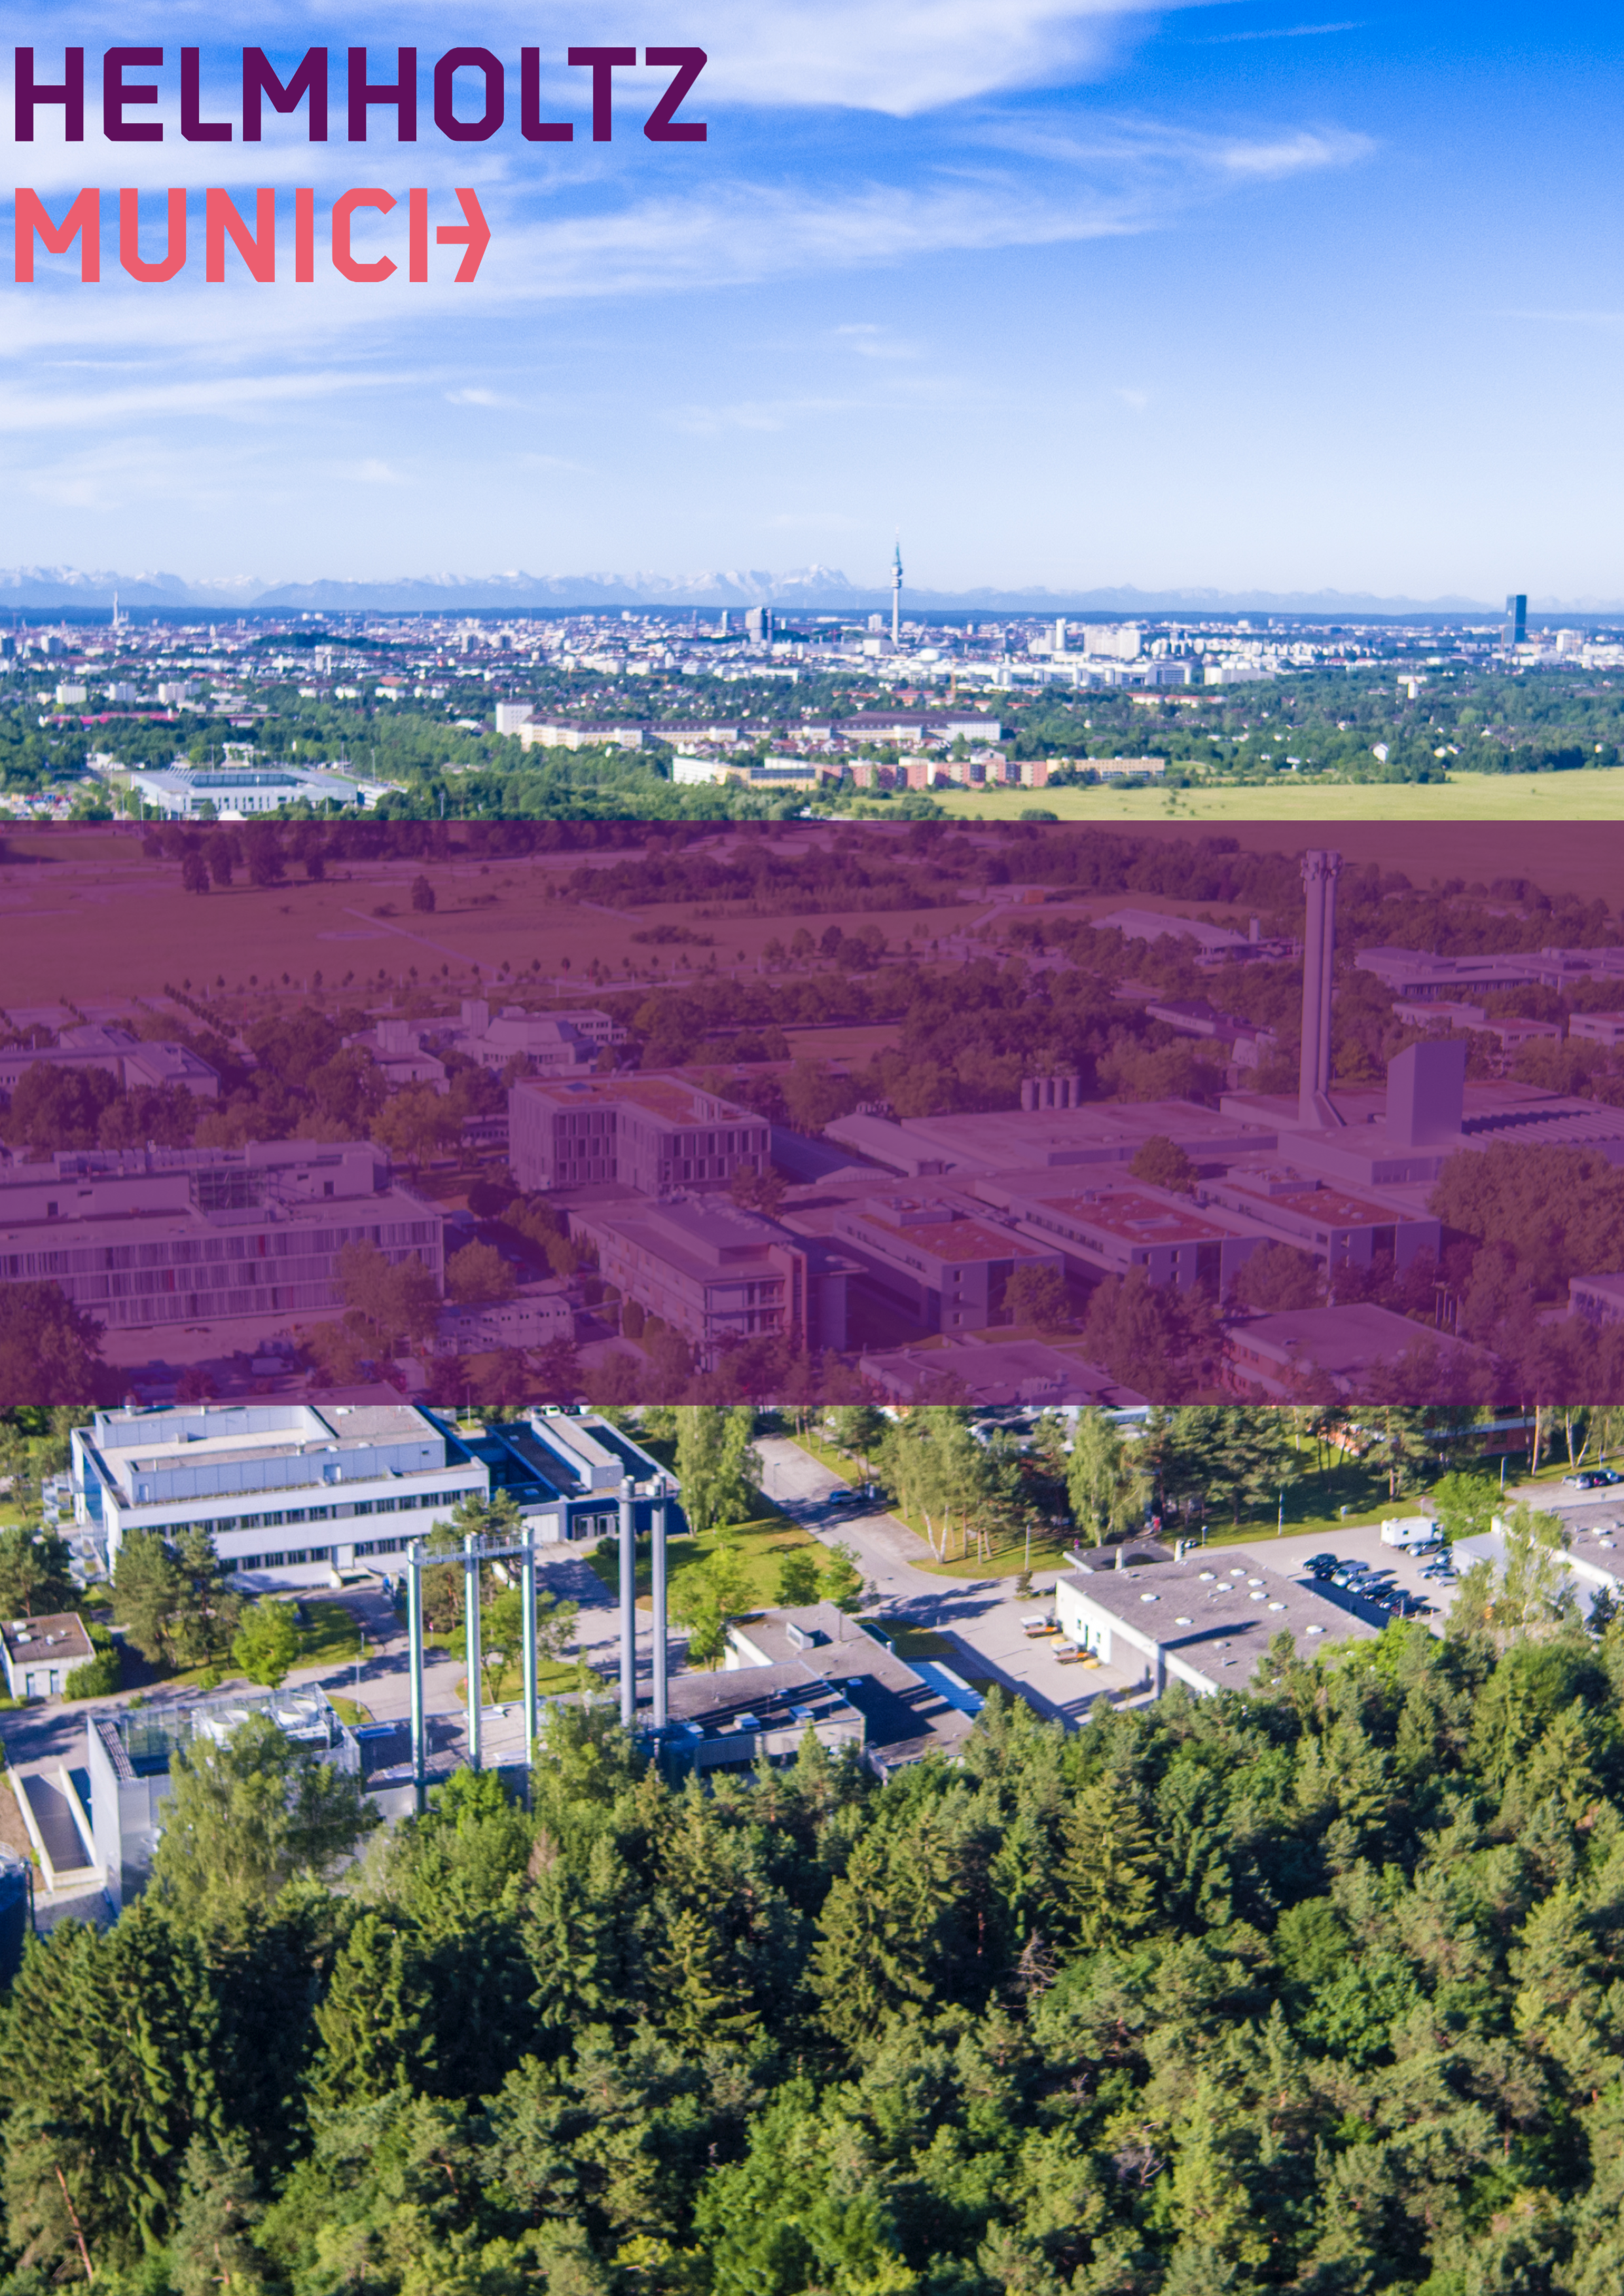
\includegraphics[width=\paperwidth,height=\paperheight]{Pictures/Book_cover_SLURM.png}}} % New Image background
\centering
\vspace*{7cm}

% Temporarily switch to Helvetica font for the title page
\usefont{T1}{phv}{b}{n}\selectfont % Helvetica Bold

\titlefont{30}{\textcolor{white}{Bioinformatics Platform}}\\ % Largest and bold

\vspace*{0.8cm}
\subtitlefont{12}{\textcolor{white}{Helmholtz Zentrum München}}\par % Smallest and normal


 \vspace*{0.8cm}

\subtitlefont{20}{\textcolor{white}{Digital Karyotyping Pipeline}}\\[0.5cm]
 \vspace*{0.08cm}
\subtitlefont{20}{\textcolor{white}{Illumina Demo Dataset Guide}}\\[0.5cm]
% Larger than Helmholtz Zentrum München, smaller than HPC TUTORIALS

\vspace*{0.8cm}
\subtitlefont{14}{\textcolor{white}{Ugur Dura}}\par % Author name

\endgroup

\normalfont

%----------------------------------------------------------------------------------------
%	COPYRIGHT PAGE
%----------------------------------------------------------------------------------------
~\vfill
% \thispagestyle{empty}

% %\noindent Copyright \copyright\ 2014 Andrea Hidalgo\\ % Copyright notice

% \noindent \textsc{Summer Research Internship, University of Western Ontario}\\

% \noindent \textsc{github.com/LaurethTeX/Clustering}\\ % URL

% \noindent This research was done under the supervision of Dr. Pauline Barmby with the financial support of the MITACS Globalink Research Internship Award within a total of 12 weeks, from June 16th to September 5th of 2014.\\ % License information

% \noindent \textit{First release, August 2014} % Printing/edition date

%----------------------------------------------------------------------------------------
%	TABLE OF CONTENTS
%----------------------------------------------------------------------------------------

\chapterimage{Pictures/Helmholtz_Zentrum_Munchen.png} % Set chapter image for TOC

\pagestyle{empty} % No headers

\tableofcontents % Print the table of contents itself

\cleardoublepage % Forces the first chapter to start on an odd page so it's on the right

\pagestyle{fancy} % Print headers again

%----------------------------------------------------------------------------------------
%	CHAPTER 1
%----------------------------------------------------------------------------------------

\chapterimage{Pictures/Helmholtz_Zentrum_Munchen.png} % Chapter heading image

\chapter{Required Software and Data}
\label{chap:required_software_and_data}

Before beginning the data extraction process, ensure you have the following software and data components installed and downloaded. This chapter provides an overview of all required tools for the Genome Studio data extraction workflow.

\section{Software Requirements}
\label{sec:software_requirements}

\subsubsection{Operating System}
\label{subsubsec:operating_system}

GenomeStudio is a Windows-only application. Ensure your system meets the following requirements:

\begin{itemize}
    \item \textbf{Operating System:} Windows 10 or Windows 11 (64-bit)
    \item \textbf{RAM:} 16 GB or more recommended for this dataset. 
    \item \textbf{Hard Disk Space:} At least 50 GB free space
\end{itemize}

\begin{tcolorbox}[colback=red!10!white,colframe=red!75!black,title=Windows Required]
\textbf{Important:} GenomeStudio only runs on Windows operating systems. macOS and Linux users will need to use a Windows virtual machine, dual-boot setup, or dedicated Windows computer to complete this tutorial.
\end{tcolorbox}

\subsubsection{GenomeStudio Software v2.0.5}
\label{subsubsec:genomestudio}

GenomeStudio is Illumina's primary software for analyzing microarray data, including genotyping, gene expression, and methylation analysis~\cite{illumina_genomestudio}.

\begin{itemize}
    \item \textbf{Version:} 2.0.5 (includes Genotyping v2.0.5 module)
    \item \textbf{Download URL:} \url{https://emea.support.illumina.com/downloads/genomestudio-2-0.html}
    \item \textbf{Release Date:} March 4, 2020
    \item \textbf{File Size:} 79 MB (ZIP archive)
    \item \textbf{Platform:} Windows 10/11 (64-bit) only
    \item \textbf{Components:}
    \begin{itemize}
        \item GenomeStudio Software v2.0.5 Installer
        \item Genotyping v2.0.5 module
        \item Polyploid Genotyping v2.0.5 module
    \end{itemize}
    \item \textbf{Documentation:} Release notes (PDF) available on the download page
\end{itemize}

\begin{tcolorbox}[colback=yellow!10!white,colframe=yellow!75!black,title=Installation Note]
GenomeStudio requires a valid license from Illumina. Contact Illumina support (\texttt{techsupport@illumina.com}) if you need assistance with licensing or installation.
\end{tcolorbox}

\subsubsection{PLINK Input Report Plug-in v2.1.4}
\label{subsubsec:plink_plugin}

The PLINK Input Report Plug-in is an essential add-on for GenomeStudio that enables export of genotyping data in PLINK format~\cite{plink_plugin,purcell2007plink,chang2015plink2}. 

\begin{itemize}
    \item \textbf{Version:} 2.1.4
    \item \textbf{Download URL:} \url{https://emea.support.illumina.com/downloads/genomestudio-2-0-plug-ins.html}
    \item \textbf{Purpose:} Export genotype data in PLINK-compatible formats (.ped, .map, .bed, .bim, .fam)
    \item \textbf{Installation:} Must be installed \textbf{after} GenomeStudio installation
\end{itemize}

\begin{tcolorbox}[colback=red!10!white,colframe=red!75!black,title=Important]
The PLINK plug-in must be installed before attempting to export data. Without this plug-in, you will not be able to generate the required output files for the Digital Karyotyping Pipeline.
\end{tcolorbox}

\newpage

%----------------------------------------------------------------------------------------
%	CHAPTER 2
%----------------------------------------------------------------------------------------
\chapterimage{Pictures/Helmholtz_Zentrum_Munchen.png} % Chapter heading image

\chapter{Downloading the Demo Dataset}
\label{chap:downloading_demo_dataset}

This chapter provides step-by-step instructions for downloading all required files for the Illumina Global Screening Array v4.0 demo dataset~\cite{illumina_gsa_datasheet,illumina_gsa_support}. The dataset consists of 36 samples and includes raw data files, manifest, cluster file, and sample sheet.

\section{Overview of Required Files}
\label{sec:overview_required_files}

The complete demo dataset consists of four main components:

\begin{enumerate}
    \item \textbf{Demo Data (iScan Raw Data)}
    \begin{itemize}
        \item 36 samples in iScan format
        \item Raw intensity data files (.idat)~\cite{illumina_infinium_assay,steemers2006infinium}
        \item Red and Green channel files for each sample
        \item Total: 72 .idat files (36 samples × 2 channels)
    \end{itemize}
    
    \item \textbf{Manifest File (BPM Format)}
    \begin{itemize}
        \item Array design and probe information
        \item Genomic coordinates (GRCh38/Build 38)~\cite{genome_reference_consortium}
        \item SNP annotations and probe sequences
        \item File: \texttt{GSA-48v4-0\_20085471\_D2.bpm}
    \end{itemize}
    
    \item \textbf{Cluster File (EGT Format)}
    \begin{itemize}
        \item Genotype cluster positions
        \item Reference population data for genotype calling
        \item Version: v4 (48v4)
        \item File: \texttt{GSA-48v4-0\_20085471\_D2\_ClusterFile.egt}
    \end{itemize}
    
    \item \textbf{Sample Sheet (CSV Format)}
    \begin{itemize}
        \item Sample metadata and identifiers
        \item Links samples to .idat files
        \item Specifies required product file versions
        \item File: \texttt{GSA-48v4-0\_D2\_SampleSheet\_Demo\_36.csv}
    \end{itemize}
\end{enumerate}

\section{Download Instructions}
\label{sec:download_instructions}

Before starting the data extraction process, you need to download the following files from Illumina's support website. All files should be downloaded and organized \textbf{before launching Genome Studio}.

\subsubsection{Step 1: Download Demo Data}
\label{subsubsec:download_demo_data}

Navigate to the Global Screening Array Support Files page:

\begin{itemize}
    \item \textbf{URL:} \url{https://emea.support.illumina.com/downloads/global-screening-array-support-files.html}
\end{itemize}

Download the following file (highlighted with red border in Figure~\ref{fig:support_files}):

\begin{enumerate}
    \item \textbf{Infinium Global Screening Array v4.0 Demo Data (iScan)}
    \begin{itemize}
        \item File format: ZIP archive
        \item Size: 825 MB
        \item Date posted: May 28, 2024
        \item Contents: 36 samples with .idat files (Red and Green channels)
        \item Total files: 72 .idat files (36 samples × 2 channels: Red and Green)
    \end{itemize}
\end{enumerate}

\begin{figure}[H]
    \centering
    \includegraphics[width=\textwidth]{images/01_Infinium_Global_Screening_Array_v4.0_support_files.png}
    \caption{Illumina Global Screening Array v4.0 Support Files page. Download the files highlighted with red borders: Demo Data (iScan) and Sample Sheet Templates.}
    \label{fig:support_files}
\end{figure}

\subsubsection{Step 2: Download Product Files and Sample Sheet}
\label{subsubsec:download_product_files}

Navigate to the Global Screening Array Product Files page:

\begin{itemize}
    \item \textbf{URL:} \url{https://emea.support.illumina.com/downloads/global-screening-array-v4-product-files.html}
\end{itemize}

Download the following files for \textbf{Build 38 (GRCh38)} (highlighted with red borders in Figure~\ref{fig:product_files}):

\begin{enumerate}
    \item \textbf{Manifest File: GSA-48v4-0\_20085471\_D2.bpm}
    \begin{itemize}
        \item File format: BPM
        \item Size: 109 MB
        \item Date posted: May 28, 2024
        \item Genome Build: GRCh38 (Build 38)
        \item \textbf{Note:} Also available in CSV format (270 MB) for reference
    \end{itemize}
    
    \item \textbf{Cluster File: GSA-48v4-0\_20085471\_D2\_ClusterFile.egt}
    \begin{itemize}
        \item File format: EGT
        \item Size: 48 MB
        \item Version: 48v4-0
        \item Date posted: May 28, 2024
    \end{itemize}
    
    \item \textbf{Sample Sheet: GSA-48v4-0\_D2\_SampleSheet\_Demo\_36.csv}
    \begin{itemize}
        \item File format: CSV
        \item Direct download: \url{https://support.illumina.com/content/dam/illumina-support/documents/documentation/chemistry_documentation/infinium_assays/infinium-gsa-with-gcra/GSA-48v4-0_20085471_D2.csv}
        \item Contains: Sample identifiers, sentrix barcodes, and product file version information
        \item Samples: 36 demo samples
    \end{itemize}
\end{enumerate}

\begin{figure}[H]
    \centering
    \includegraphics[width=\textwidth]{images/02_Infinium_Global_Screening_Array_v4.0_product_files.png}
    \caption{Illumina Global Screening Array v4.0 Product Files page. Download the files highlighted with red borders: Manifest File Build 38 (BPM Format), Cluster File (EGT Format), and Sample Sheet (CSV). The sample sheet can also be downloaded directly from the provided URL.}
    \label{fig:product_files}
\end{figure}

\begin{tcolorbox}[colback=blue!5!white,colframe=blue!75!black,title=Important Note]
Since the demo data is based on \textbf{GRCh38 (Build 38)}, ensure you download the corresponding manifest and cluster files for Build 38. Using mismatched genome builds will result in incorrect genomic coordinates and analysis errors. The sample sheet (\texttt{GSA-48v4-0\_D2\_SampleSheet\_Demo\_361.csv}) specifies the exact product file versions required for this dataset.
\end{tcolorbox}

\subsubsection{Step 3: Organize Downloaded Files}
\label{subsubsec:organize_files}

Create a dedicated directory on your Desktop to organize all files. Follow this structure:

\begin{enumerate}
    \item Create the main directory:
    \begin{lstlisting}[style=bashstyle]
Desktop/
`-- Infinium_Global_Screening_Array_v4.0/
    \end{lstlisting}
    
    \item Extract and organize the downloaded files under the \textbf{Infinium\_Global\_Screening\_Array\_v4.0} folder (the name of the folder is arbitrary, you can choose any name you want); 
    \begin{lstlisting}[style=bashstyle]
Infinium_Global_Screening_Array_v4.0/
|-- idats_Demo_36/
|   |-- 204939850001_R01C01_Red.idat
|   |-- 204939850001_R01C01_Grn.idat
|   |-- 204939850001_R01C02_Red.idat
|   |-- 204939850001_R01C02_Grn.idat
|   `-- ... (36 samples = 72 .idat files total)
|-- GSA-48v4-0_20085471_D2.bpm
|-- GSA-48v4-0_20085471_D2_ClusterFile.egt
`-- GSA-48v4-0_D2_SampleSheet_Demo_36.csv
    \end{lstlisting}
\end{enumerate}

\section{Pre-Analysis Checklist}
\label{sec:pre_analysis_checklist}

Before proceeding to create a genotyping project in Genome Studio, verify you have completed all the following steps:

\begin{table}[h]
\centering
\begin{tabular}{|p{10cm}|c|}
\hline
\textbf{Item} & \textbf{Status} \\
\hline
\multicolumn{2}{|c|}{\textbf{Software Installation}} \\
\hline
GenomeStudio v2.0.5 installed & $\square$ \\
\hline
GenomeStudio license activated & $\square$ \\
\hline
PLINK Input Report Plug-in v2.1.4 installed & $\square$ \\
\hline
\multicolumn{2}{|c|}{\textbf{Data Downloaded}} \\
\hline
Demo data downloaded (36 samples, 72 .idat files) & $\square$ \\
\hline
Manifest file: GSA-48v4-0\_20085471\_D2.bpm & $\square$ \\
\hline
Cluster file: GSA-48v4-0\_20085471\_D2\_ClusterFile.egt & $\square$ \\
\hline
Sample sheet: GSA-48v4-0\_D2\_SampleSheet\_Demo\_36.csv & $\square$ \\
\hline
\multicolumn{2}{|c|}{\textbf{Data Organization}} \\
\hline
All files organized in dedicated directory structure & $\square$ \\
\hline
iScan raw data extracted from ZIP archive & $\square$ \\
\hline
File paths are accessible and correct & $\square$ \\
\hline
\end{tabular}
\caption{Pre-analysis checklist - Complete before starting Genome Studio}
\label{tab:pre_analysis_checklist}
\end{table}

\begin{tcolorbox}[colback=green!5!white,colframe=green!75!black,title=Ready to Begin Genome Studio Analysis]
Once all items in the checklist above are completed, you are ready to proceed with creating a genotyping project in Genome Studio. The next section will guide you through the step-by-step process of project creation, genotype calling, and data extraction.
\end{tcolorbox}


\newpage

%----------------------------------------------------------------------------------------
%	CHAPTER 3
%----------------------------------------------------------------------------------------
\chapterimage{Pictures/Helmholtz_Zentrum_Munchen.png} % Chapter heading image

\chapter{Data Extraction with Genome Studio}
\label{chap:data_extraction}

This chapter provides detailed step-by-step instructions for extracting the required data files from Genome Studio. These files are essential inputs for the Digital Karyotyping Pipeline and include genotype data, sample information, SNP annotations, and PLINK format files.

\section{Overview of Required Output Files}
\label{sec:required_output_files}

The Digital Karyotyping Pipeline requires the following files to be extracted from Genome Studio:

\begin{enumerate}
    \item \textbf{Full Data Table} (\texttt{Full\_Data\_Table.txt})
    \begin{itemize}
        \item Contains comprehensive genotyping data for all samples and SNPs
        \item Includes LRR (Log R Ratio) and BAF (B Allele Frequency) values~\cite{lrr_baf_analysis}
        \item Critical for copy number variation (CNV) analysis~\cite{cnv_detection}
    \end{itemize}
    
    \item \textbf{Samples Table} (\texttt{Samples\_Table.txt})
    \begin{itemize}
        \item Contains sample-level quality control metrics
        \item Includes call rates, heterozygosity~\cite{roh_detection}, and other QC parameters
        \item Used for sample quality assessment
    \end{itemize}
    
    \item \textbf{SNP Table} (\texttt{SNP\_Table.txt})
    \begin{itemize}
        \item Contains SNP-level information and statistics
        \item Includes genomic coordinates and allele frequencies
        \item Used for marker quality control
    \end{itemize}
    
    \item \textbf{PLINK Files} (\texttt{.ped}, \texttt{.map}, \texttt{.bed}, \texttt{.bim}, \texttt{.fam})
    \begin{itemize}
        \item Standard genetic data format for downstream analysis~\cite{purcell2007plink,chang2015plink2}
        \item Generated using PLINK Input Report Plug-in~\cite{plink_plugin}
        \item Required for genotype-based analyses
    \end{itemize}
    
    \item \textbf{Manifest File} (\texttt{GSA-48v4-0\_20085471\_D2.csv})
    \begin{itemize}
        \item Array design information in CSV format
        \item Already downloaded in section \ref{subsubsec:download_product_files}
        \item Contains probe annotations and genomic coordinates
    \end{itemize}
\end{enumerate}

\begin{tcolorbox}[colback=yellow!10!white,colframe=yellow!75!black,title=Important: Folder Structure,breakable]
    Make sure your folder structure is organized as follows before starting:
    \begin{itemize}
        \item \textbf{Sample Sheet:} 
        
        \texttt{\small Infinium\_Global\_Screening\_Array\_v4.0/}\\\texttt{\small GSA-48v4-0\_D2\_SampleSheet\_Demo\_36.csv}
        
        \item \textbf{Data Repository:} 
        
        \texttt{\small Infinium\_Global\_Screening\_Array\_v4.0/idats\_Demo\_36/}
        
        (contains .idat files)
        
        \item \textbf{Manifest Repository:} 
        
        \texttt{\small Infinium\_Global\_Screening\_Array\_v4.0/}
        
        (contains .bpm and .egt files)
    \end{itemize}
    All three paths should point to locations within or at the \texttt{\small Infinium\_Global\_Screening\_Array\_v4.0/} directory.
    \end{tcolorbox}

    


\section{Step 1: Creating a Genotyping Project}
\label{sec:creating_genotyping_project}

\subsection{Launch Genome Studio}
\label{subsec:launch_genomestudio}

\begin{enumerate}
    \item Open Genome Studio v2.0.5 from the Windows Start menu
    \item Wait for the application to fully load
    \item You will see the Genome Studio welcome screen
\end{enumerate}

\subsection{Start New Genotyping Project}
\label{subsec:start_new_project}

\begin{enumerate}
    \item Click on \textbf{File} → \textbf{New Project} (see Figure~\ref{fig:open_new_project})
    \item Select \textbf{Genotyping} from the project type options
    \item The Genotyping Wizard will open (see Figure~\ref{fig:genotyping_wizard})
\end{enumerate}

\begin{figure}[H]
    \centering
    \includegraphics[width=\textwidth]{images/03_open_new_project.png}
    \caption{Creating a new genotyping project. Select File → New Project → Genotyping to launch the Genotyping Wizard.}
    \label{fig:open_new_project}
\end{figure}

\begin{figure}[H]
    \centering
    \includegraphics[width=\textwidth]{images/04_gnotyping_wizard.png}
    \caption{The Genotyping Wizard guides you through the project setup process, including project naming, sample sheet import, data repository selection, and manifest loading.}
    \label{fig:genotyping_wizard}
\end{figure}

\subsection{Name Your Project}
\label{subsec:name_project}

The first step in the Genotyping Wizard is to name your project and choose where to save it.

\begin{enumerate}
    \item Enter a descriptive project name (e.g., \texttt{Infinium\_Global\_Screening\_Array}) (see Figure~\ref{fig:project_naming2})
    \item Choose a location to save the project file (.bsc)
    \item Recommended location: \texttt{Infinium\_Global\_Screening\_Array\_v4.0/GenomeStudio\_Project/}
    \item Click \textbf{Next} to proceed to the next step
\end{enumerate}

\begin{figure}[H]
    \centering
    \includegraphics[width=\textwidth]{images/05_genotyping_project_naming2.png}
    \caption{Entering the project name and selecting the save location. Use a descriptive name that reflects the dataset (e.g., Infinium\_Global\_Screening\_Array).}
    \label{fig:project_naming2}
\end{figure}

\subsection{Specify Data and Manifest Repositories}
\label{subsec:specify_repositories}

After naming your project, the wizard will ask you to specify how to load your samples and where to find the necessary files. This step involves three key inputs: the sample sheet, the data repository (where .idat files are located), and the manifest repository (where .bpm and .egt files are located).

\subsubsection{Select Sample Loading Method}
\label{subsubsec:select_sample_loading}

First, you need to tell Genome Studio how you want to load your samples.

\begin{enumerate}
    \item The wizard will display: \textit{"Please specify the samples you want to load by identifying the sample sheet and associated data and manifest repositories"}
    \item Select \textbf{Use sample sheet to load sample intensities} (see Figure~\ref{fig:use_samplesheet})
    \item Click \textbf{Next} to proceed to the repository specification screen
\end{enumerate}

\begin{figure}[H]
    \centering
    \includegraphics[width=\textwidth]{images/06_genotyping_wizard_use_samplesheet.png}
    \caption{Selecting the sample loading method. Choose "Use sample sheet to load sample intensities" to link sample identifiers to their corresponding .idat files using a CSV sample sheet.}
    \label{fig:use_samplesheet}
\end{figure}

\subsubsection{Provide Sample Sheet Path}
\label{subsubsec:provide_sample_sheet}

After clicking Next, you will see three input fields for specifying file locations. Start with the sample sheet.

\begin{enumerate}
    \item In the \textbf{Sample Sheet} field, click \textbf{Browse} (see Figure~\ref{fig:input_files})
    \item Navigate to: \texttt{Infinium\_Global\_Screening\_Array\_v4.0/}
    \item Select the file: \texttt{GSA-48v4-0\_D2\_SampleSheet\_Demo\_36.csv}
    \item Click \textbf{Open}
    \item The path will appear in the Sample Sheet field
\end{enumerate}

\begin{figure}[H]
    \centering
    \includegraphics[width=\textwidth]{images/07_genotyping_wizard_input_files.png}
    \caption{Specifying the sample sheet location. Click Browse next to the Sample Sheet field and select the CSV file (GSA-48v4-0\_D2\_SampleSheet\_Demo\_36.csv). This file contains the mapping between sample identifiers and their corresponding .idat files.}
    \label{fig:input_files}
\end{figure}

\subsubsection{Provide Data Repository Path}
\label{subsubsec:provide_data_repository}

Next, specify where your .idat files (raw intensity data) are located.

\begin{enumerate}
    \item In the \textbf{Data Repository} field, click \textbf{Browse} (see Figure~\ref{fig:data_repo_selection})
    \item Navigate to: \texttt{Infinium\_Global\_Screening\_Array\_v4.0/}
    \item Select the folder: \texttt{idats\_Demo\_36/}
    \item Click \textbf{Select Folder} or \textbf{OK}
    \item The path will appear in the Data Repository field
    \item This folder contains all 72 .idat files (36 samples × 2 channels: Red and Green)
\end{enumerate}

\begin{figure}[H]
    \centering
    \includegraphics[width=\textwidth]{images/08_genotyping_wizard_data_repo_selection.png}
    \caption{Specifying the data repository location. Click Browse next to the Data Repository field and select the folder containing your .idat files (idats\_Demo\_36/). This folder should contain 72 .idat files: 36 Red channel files and 36 Green channel files.}
    \label{fig:data_repo_selection}
\end{figure}

\subsubsection{Provide Manifest Repository Path}
\label{subsubsec:provide_manifest_repository}

Finally, specify where your manifest (.bpm) and cluster (.egt) files are located.

\begin{enumerate}
    \item In the \textbf{Manifest Repository} field, click \textbf{Browse} (see Figure~\ref{fig:manifest_selection})
    \item Navigate to and select the folder: \texttt{Infinium\_Global\_Screening\_Array\_v4.0/}
    \item Click \textbf{Select Folder} or \textbf{OK}
    \item The path will appear in the Manifest Repository field
    \item This folder should contain:
    \begin{itemize}
        \item \texttt{GSA-48v4-0\_20085471\_D2.bpm} (manifest file)
        \item \texttt{GSA-48v4-0\_20085471\_D2\_ClusterFile.egt} (cluster file)
    \end{itemize}
    \item Verify that all three paths (Sample Sheet, Data Repository, Manifest Repository) are correctly specified
    \item Click \textbf{Next} to proceed to cluster file configuration
\end{enumerate}

\begin{figure}[H]
    \centering
    \includegraphics[width=\textwidth]{images/09_genotyping_wizard_input_manifes_selection.png}
    \caption{Specifying the manifest repository location. Click Browse next to the Manifest Repository field and select the folder (Infinium\_Global\_Screening\_Array\_v4.0/) that contains both the manifest file (GSA-48v4-0\_20085471\_D2.bpm) and cluster file (GSA-48v4-0\_20085471\_D2\_ClusterFile.egt). It is normal not to see .bpm and .egt files in the select folder dialog since it is asking for the parent directory. After verifying all three paths, click Next.}
    \label{fig:manifest_selection}
\end{figure}

\subsection{Configure Cluster File and Analysis Settings}
\label{subsec:configure_cluster_file}

After specifying all repository paths, you need to configure the cluster file and analysis settings.

\begin{enumerate}
    \item On the Cluster File Configuration page, check the box for \textbf{Import cluster positions from a cluster file} (see Figure~\ref{fig:cluster_selection})
    \item Click \textbf{Browse} to select the cluster file
    \item Navigate to the \texttt{Infinium\_Global\_Screening\_Array\_v4.0/} folder
    \item Select the file: \texttt{GSA-48v4-0\_20085471\_D2\_ClusterFile.egt}
    \item Click \textbf{Open}
    \item Verify the following settings:
    \begin{itemize}
        \item \textbf{GenCall Threshold:} 0.15 (default, recommended value)
        \item \textbf{Calculate Sample and SNP Statistics:} Checked (enabled)
    \end{itemize}
    \item Click \textbf{Finish} to start the genotype calling process (see Figure~\ref{fig:finish_button})
\end{enumerate}

\begin{figure}[H]
    \centering
    \includegraphics[width=\textwidth]{images/10_cluster_files_selection.png}
    \caption{Cluster file configuration page. Check "Import cluster positions from a cluster file" and browse to select GSA-48v4-0\_20085471\_D2\_ClusterFile.egt from your working directory. Ensure GenCall Threshold is set to 0.15 and "Calculate Sample and SNP Statistics" is checked.}
    \label{fig:cluster_selection}
\end{figure}

\begin{figure}[H]
    \centering
    \includegraphics[width=\textwidth]{images/11_finish_button.png}
    \caption{Final confirmation page. After verifying all settings including cluster file selection, GenCall threshold (0.15), and statistics calculation option, click Finish to begin the genotype calling process.}
    \label{fig:finish_button}
\end{figure}

\begin{tcolorbox}[colback=blue!10!white,colframe=blue!75!black,title=Important Settings]
\textbf{GenCall Threshold (0.15):} This threshold determines the minimum quality score required for a genotype call to be considered valid. The default value of 0.15 is recommended for most applications.

\textbf{Calculate Sample and SNP Statistics:} This option must be enabled to generate quality control metrics (call rates, heterozygosity, Hardy-Weinberg equilibrium, etc.) that are essential for data quality assessment.
\end{tcolorbox}

\subsection{Genotype Calling Process}
\label{subsec:genotype_calling}

After clicking Finish, Genome Studio will begin processing the data automatically.

\begin{enumerate}
    \item The software will display a loading screen (see Figure~\ref{fig:loading_screen})
    \item Genome Studio will:
    \begin{itemize}
        \item Load all .idat files from the data repository
        \item Apply the cluster file for genotype calling
        \item Calculate quality metrics (call rates, GC scores, heterozygosity)
        \item Generate intensity plots and cluster plots
        \item Compute sample and SNP statistics
    \end{itemize}
    \item This process may take 10-30 minutes depending on your system specifications
    \item A progress bar will show the analysis status
    \item Wait for the process to complete before proceeding to the next step
\end{enumerate}

\begin{figure}[H]
    \centering
    \includegraphics[width=\textwidth]{images/12_loading_screen.png}
    \caption{Genome Studio loading screen during data processing. The software is reading .idat files, applying the cluster file, and performing genotype calling. This may take 10-30 minutes for 36 samples.}
    \label{fig:loading_screen}
\end{figure}


Once the genotype calling process is complete, Genome Studio will prompt you to update quality metrics.

\subsection{Update Heritability and Reproducibility Errors}
\label{subsec:update_heritability}

After the initial data processing completes, Genome Studio will display a dialog asking about updating quality metrics.

\begin{enumerate}
    \item A dialog will appear with the message: \textit{"Do you wish to update all heritability and reproducibility errors? This operation may take some time."} (see Figure~\ref{fig:heritability_prompt})
    \item Click \textbf{Yes} to update these quality metrics
    \item A progress bar will appear showing the calculation status (see Figure~\ref{fig:heritability_progress})
    \item This process typically takes 5-10 minutes for 36 samples
    \item Wait for the process to complete before proceeding
\end{enumerate}

\begin{figure}[H]
    \centering
    \includegraphics[width=\textwidth]{images/13_herritability_errors_yes.png}
    \caption{Heritability and reproducibility error update prompt. Click Yes to calculate these quality metrics, which are important for assessing data reliability and identifying potential technical issues.}
    \label{fig:heritability_prompt}
\end{figure}

\begin{figure}[H]
    \centering
    \includegraphics[width=\textwidth]{images/14_heritability_error_progress_bar.png}
    \caption{Progress bar showing the calculation of heritability and reproducibility errors. This process analyzes replicate samples and family relationships to compute quality metrics. Wait for completion before proceeding.}
    \label{fig:heritability_progress}
\end{figure}

\begin{tcolorbox}[colback=blue!10!white,colframe=blue!75!black,title=About Heritability and Reproducibility Errors]
\textbf{Heritability Errors:} Measure the consistency of genotype calls across related samples (parent-offspring, siblings). High heritability errors may indicate genotyping quality issues.

\textbf{Reproducibility Errors:} Measure the consistency of genotype calls across technical replicates of the same sample. Low reproducibility indicates poor technical quality.

These metrics are essential for quality control and should always be calculated.
\end{tcolorbox}

Once the heritability and reproducibility error calculations are complete, Genome Studio will display the main genotyping interface with multiple data views (see Figure~\ref{fig:initial_screen}).

\begin{figure}[H]
    \centering
    \includegraphics[width=\textwidth]{images/15_initial_screen.png}
    \caption{Genome Studio genotyping module interface after successful project loading and quality metrics calculation. The interface shows multiple tabs including Full Data Table, SNP Table, and Samples Table, which contain all the genotyping results and quality metrics.}
    \label{fig:initial_screen}
\end{figure}

\section{Step 2: Full Data Table Column Configuration}
\label{sec:full_data_table_columns}

After the genotype calling is complete, you need to configure the columns in the Full Data Table to ensure all required data fields are included for export.

\subsection{Access Full Data Table View}
\label{subsec:access_full_data_table}

\begin{enumerate}
    \item Once genotype calling is complete, navigate to the \textbf{Full Data Table} tab
    \item This table displays all genotyping data in a spreadsheet format
    \item By default, not all columns are visible
\end{enumerate}

\subsection{Configure Required Columns}
\label{subsec:configure_columns}

\begin{enumerate}
    \item Right-click on the column header area (see Figure~\ref{fig:columns_chooser})
    \item Select \textbf{Choose Columns} or \textbf{Column Chooser}
    \item A dialog box will appear with available columns on the right (Hidden Columns) and selected columns on the left (Shown Columns)
\end{enumerate}

\begin{figure}[H]
    \centering
    \includegraphics[width=\textwidth]{images/16_columns_chooser.png}
    \caption{Opening the Column Chooser dialog. This allows you to select which data fields to include in the Full Data Table export.}
    \label{fig:columns_chooser}
\end{figure}

\subsection{Select Essential Columns}
\label{subsec:select_columns}

Ensure the following columns are selected for the Digital Karyotyping Pipeline. The most critical columns are \textbf{B Allele Freq} and \textbf{Log R Ratio}:

\begin{table}[h]
\centering
\small
\begin{tabular}{|l|p{8cm}|}
\hline
\textbf{Column Name} & \textbf{Description} \\
\hline
Index & Row index number \\
\hline
Name & Marker identifier (rsID or probe name) \\
\hline
Address & Probe address on the array \\
\hline
Chr & Chromosome \\
\hline
Position & Genomic position (bp) \\
\hline
GenTrain Score & Cluster quality score \\
\hline
Frac A & Fraction of A allele \\
\hline
Frac C & Fraction of C allele \\
\hline
Frac G & Fraction of G allele \\
\hline
Frac T & Fraction of T allele \\
\hline
GType & Genotype call \\
\hline
Score & Genotype quality score \\
\hline
Theta & Normalized angle (allelic ratio) \\
\hline
R & Normalized intensity (total signal) \\
\hline
B Allele Freq & B Allele Frequency (BAF)~\cite{lrr_baf_analysis} \\
\hline
Log R Ratio & Log R Ratio (LRR)~\cite{lrr_baf_analysis} \\
\hline
\end{tabular}
\caption{Essential columns required for the Full Data Table export}
\label{tab:required_columns}
\end{table}

\subsubsection{Adding B Allele Freq Column}

\begin{enumerate}
    \item In the Column Chooser dialog, locate \textbf{B Allele Freq} in the right panel (Hidden Columns)
    \item Select \textbf{B Allele Freq} (see Figure~\ref{fig:columns_chooser1})
    \item Click the \textbf{Show} button to move it to the left panel (Shown Columns)
\end{enumerate}

\begin{figure}[H]
    \centering
    \includegraphics[width=\textwidth]{images/17_columns_chooser1.png}
    \caption{Selecting B Allele Freq from the Hidden Columns panel. Click the Show button to add it to the visible columns in the Full Data Table.}
    \label{fig:columns_chooser1}
\end{figure}

\subsubsection{Adding Log R Ratio Column}

\begin{enumerate}
    \item In the Column Chooser dialog, locate \textbf{Log R Ratio} in the right panel (Hidden Columns)
    \item Select \textbf{Log R Ratio} (see Figure~\ref{fig:columns_chooser_w})
    \item Click the \textbf{Show} button to move it to the left panel (Shown Columns)
    \item Click \textbf{OK} to apply the column configuration
\end{enumerate}

\begin{figure}[H]
    \centering
    \includegraphics[width=\textwidth]{images/18_columns_chooser_w.png}
    \caption{Selecting Log R Ratio from the Hidden Columns panel. After clicking Show, click OK to apply all column changes to the Full Data Table.}
    \label{fig:columns_chooser_w}
\end{figure}

\begin{tcolorbox}[colback=red!10!white,colframe=red!75!black,title=Critical Step]
\textbf{Important:} Ensure all columns in Table~\ref{tab:required_columns} are selected before exporting. Missing columns will cause errors in the Digital Karyotyping Pipeline. Pay special attention to:
\begin{itemize}
    \item B Allele Freq (BAF) - Required for CNV detection
    \item Log R Ratio (LRR) - Required for copy number analysis
    \item Chr and Position - Required for genomic mapping
\end{itemize}
\end{tcolorbox}

\section{Step 3: Exporting Data Tables}
\label{sec:exporting_data_tables}

Now that the project is created and columns are configured, you can export the required data tables for the Digital Karyotyping Pipeline.

\subsection{Export Full Data Table}
\label{subsec:export_full_data_table}

After configuring all required columns, you can now export the Full Data Table.

\subsubsection{Create Data Directory}

Before exporting, create a \texttt{data/} directory within your project folder to organize all exported files:

\begin{lstlisting}
Infinium_Global_Screening_Array_v4.0/
|-- GSA-48v4-0_20085471_D2.bpm
|-- GSA-48v4-0_20085471_D2_ClusterFile.egt
|-- GSA-48v4-0_D2_SampleSheet_Demo_36.csv
|-- idats_Demo_36/
`-- data/                          <- Create this directory
    `-- Full_Data_Table.txt        <- Export files here
\end{lstlisting}

\subsubsection{Export Process}

\begin{enumerate}
    \item In the Full Data Table view, click the \textbf{Export Data} button in the toolbar (see Figure~\ref{fig:full_data_table})
    \item A file save dialog will appear
    \item Navigate to the \texttt{data/} directory you created under your project folder
    \item Save as: \texttt{Full\_Data\_Table.txt}
    \item Click \textbf{Save}
\end{enumerate}

\begin{figure}[H]
    \centering
    \includegraphics[width=\textwidth]{images/19_fulll_data_Table_extraction.png}
    \caption{Clicking the Export Data button in the Full Data Table view and selecting the save location. Navigate to the \texttt{data/} directory within your project folder and save the file as \texttt{Full\_Data\_Table.txt}.}
    \label{fig:full_data_table}
\end{figure}

\subsubsection{Export Confirmation}

\begin{enumerate}
    \item After clicking Save, a dialog will appear asking: \textit{"Currently, only the selected rows and columns will be exported. Would you prefer to Export the entire table?"} (see Figure~\ref{fig:full_data_export1})
    \item Click \textbf{Yes} to export the entire table (all samples and all SNPs)
    \item The export process will begin (see Figure~\ref{fig:full_data_export2} for progress)
\end{enumerate}

\begin{figure}[H]
    \centering
    \includegraphics[width=\textwidth]{images/20_fulll_data_Table_extraction_1.png}
    \caption{Export confirmation dialog. Click Yes to export the entire Full Data Table including all samples and SNPs with all configured columns.}
    \label{fig:full_data_export1}
\end{figure}

\begin{figure}[H]
    \centering
    \includegraphics[width=\textwidth]{images/21_fulll_data_Table_extraction_2.png}
    \caption{Full Data Table export progress bar. The export may take several minutes depending on the dataset size (36 samples × ~700,000 SNPs for this demo).}
    \label{fig:full_data_export2}
\end{figure}

\begin{tcolorbox}[colback=green!10!white,colframe=green!75!black,title=Export Time Estimate]
The Full Data Table export typically takes:
\begin{itemize}
    \item \textbf{Demo dataset (36 samples):} 5-10 minutes
    \item \textbf{Larger datasets (100+ samples):} 15-30 minutes
    \item File size: Approximately 1-2 GB for this demo dataset
\end{itemize}
Do not close Genome Studio during the export process.
\end{tcolorbox}

\subsection{Export SNP Table}
\label{subsec:export_snp_table}

After exporting the Full Data Table, you need to export the SNP Table which contains marker-level statistics.

\begin{enumerate}
    \item Navigate to the \textbf{SNP Table} tab in Genome Studio
    \item Click the \textbf{Export Data} button in the toolbar (see Figure~\ref{fig:snp_table_export})
    \item A file save dialog will appear
    \item Navigate to the \texttt{data/} directory (same location as Full Data Table)
    \item Save as: \texttt{SNP\_Table.txt}
    \item Click \textbf{Save}
    \item A dialog will appear asking: \textit{"Would you prefer to Export the entire table?"}
    \item Click \textbf{Yes} to export all SNPs with all statistics
    \item The export process will begin (see Figure~\ref{fig:snp_table_progress} for export progress)
\end{enumerate}

\begin{figure}[H]
    \centering
    \includegraphics[width=\textwidth]{images/22_SNP_Table_extraction.png}
    \caption{Exporting the SNP Table. Click the Export Data button in the SNP Table tab and save to the \texttt{data/} directory. This table contains marker-level statistics including call rates, allele frequencies, and Hardy-Weinberg equilibrium p-values.}
    \label{fig:snp_table_export}
\end{figure}

\begin{figure}[H]
    \centering
    \includegraphics[width=\textwidth]{images/23_SNP_Table_extraction_progress.png}
    \caption{Export progress indicator for SNP Table. The export typically takes 2-5 minutes for ~700,000 SNPs.}
    \label{fig:snp_table_progress}
\end{figure}

\subsection{Export Samples Table}
\label{subsec:export_samples_table}

Finally, export the Samples Table which contains sample-level quality control metrics.

\begin{enumerate}
    \item Navigate to the \textbf{Samples Table} tab in Genome Studio
    \item Click the \textbf{Export Data} button in the toolbar (see Figure~\ref{fig:samples_table_export})
    \item A file save dialog will appear
    \item Navigate to the \texttt{data/} directory (same location as previous exports)
    \item Save as: \texttt{Samples\_Table.txt}
    \item Click \textbf{Save}
    \item A dialog will appear asking: \textit{"Would you prefer to Export the entire table?"}
    \item Click \textbf{Yes} to export all samples with all QC metrics
    \item The export completes quickly (typically under 1 minute for 36 samples)
\end{enumerate}

\begin{figure}[H]
    \centering
    \includegraphics[width=\textwidth]{images/24_Sample_table_extraction.png}
    \caption{Exporting the Samples Table. Click the Export Data button in the Samples Table tab and save to the \texttt{data/} directory. This table contains sample-level QC metrics (call rates, heterozygosity, etc.) essential for quality control and filtering.}
    \label{fig:samples_table_export}
\end{figure}

\begin{tcolorbox}[colback=green!10!white,colframe=green!75!black,title=Data Export Complete]
After exporting all three tables, your \texttt{data/} directory should contain:
\begin{itemize}
    \item \texttt{Full\_Data\_Table.txt} - Complete genotyping data with LRR and BAF
    \item \texttt{SNP\_Table.txt} - Marker-level statistics and QC metrics
    \item \texttt{Samples\_Table.txt} - Sample-level QC metrics
\end{itemize}
These three files are required inputs for the Digital Karyotyping Pipeline.
\end{tcolorbox}

\begin{figure}[H]
    \centering
    \includegraphics[width=0.8\textwidth]{images/25_extracted_data.png}
    \caption{Contents of the \texttt{data/} directory after exporting all three tables (Full Data Table, SNP Table, and Samples Table). These are the core Genome Studio exports required for the pipeline.}
    \label{fig:extracted_data_tables}
\end{figure}

\begin{tcolorbox}[colback=green!5!white,colframe=green!75!black,title=Export Tips]
\textbf{Best Practices for Data Export:}
\begin{itemize}
    \item Create a dedicated \texttt{./data/} folder for all output files
    \item Verify file sizes after export (Full Data Table should be largest)
\end{itemize}
\end{tcolorbox}

\subsection{Export Process}



\section{Step 4: Generating PLINK Files}
\label{sec:generating_plink_files}

The final step is to generate PLINK format files using the PLINK Input Report Plug-in v2.1.4 installed in Chapter 1. This plug-in converts Genome Studio genotyping data into PLINK-compatible formats (.ped, .map, .bed, .bim, .fam) required by the Digital Karyotyping Pipeline.

\subsection{Access Report Wizard}
\label{subsec:access_plink_report}

\begin{enumerate}
    \item In Genome Studio, go to \textbf{Analysis} → \textbf{Reports} → \textbf{Report Wizard} (see Figure~\ref{fig:plink_wizard})
    \item The Report Wizard window will open with several report options
\end{enumerate}

\begin{figure}[H]
    \centering
    \includegraphics[width=\textwidth]{images/26_plink_report_wizard.png}
    \caption{Accessing the Report Wizard. Click on Analysis → Reports → Report Wizard to open the report generation interface.}
    \label{fig:plink_wizard}
\end{figure}

\subsection{Select PLINK Input Report}
\label{subsec:select_plink_report}

\begin{enumerate}
    \item In the Report Wizard window, you will see several report options (see Figure~\ref{fig:plink_wizard2})
    \item Under the \textbf{Custom Reports} section, select \textbf{PLINK Input Report 2.1.4}
    \begin{itemize}
        \item If you do not see PLINK in the list, verify that the PLINK Input Report Plug-in was installed correctly (see Chapter 1)
    \end{itemize}
    \item Click \textbf{Next} to proceed
\end{enumerate}

\begin{figure}[H]
    \centering
    \includegraphics[width=\textwidth]{images/27_plink_report_wizard_2.png}
    \caption{Selecting PLINK Input Report from the Custom Reports section. The version shown should be 2.1.4 if the plug-in was installed correctly.}
    \label{fig:plink_wizard2}
\end{figure}

\subsection{Select Samples to Include}
\label{subsec:select_samples}

\begin{enumerate}
    \item The wizard will ask: \textit{"Which samples would you like to include in your report?"} (see Figure~\ref{fig:plink_wizard3})
    \item Select \textbf{All samples}
    \item Click \textbf{Next} to proceed
\end{enumerate}

\begin{figure}[H]
    \centering
    \includegraphics[width=\textwidth]{images/28_plink_report_wizard_3.png}
    \caption{Selecting samples for PLINK export. Choose "All samples" to include all 36 demo samples in the output.}
    \label{fig:plink_wizard3}
\end{figure}

\subsection{Select Sample Groups}
\label{subsec:select_sample_groups}

\begin{enumerate}
    \item The wizard will ask: \textit{"This project has various sample groups. Please select the ones you want to include in the report."} (see Figure~\ref{fig:plink_wizard4})
    \item Select \textbf{all available options}:
    \begin{itemize}
        \item CEU
        \item CEU\_Rep
        \item CEU\_Unrel
    \end{itemize}
    \item Click \textbf{Next} to proceed
\end{enumerate}

\begin{figure}[H]
    \centering
    \includegraphics[width=\textwidth]{images/29_plink_report_wizard_4.png}
    \caption{Selecting sample groups for PLINK export. Choose all available groups (CEU, CEU\_Rep, and CEU\_Unrel) to include all samples.}
    \label{fig:plink_wizard4}
\end{figure}

\subsection{Select SNPs to Include}
\label{subsec:select_snps}

\begin{enumerate}
    \item The wizard will ask: \textit{"Which SNPs would you like to include in your report?"} (see Figure~\ref{fig:plink_wizard5})
    \item Select \textbf{Include zeroed SNPs in the report}
    \begin{itemize}
        \item This ensures all SNPs are included, even those with zero intensity values
    \end{itemize}
    \item Click \textbf{Next} to proceed
\end{enumerate}

\begin{figure}[H]
    \centering
    \includegraphics[width=\textwidth]{images/30_plink_report_wizard_5.png}
    \caption{Selecting SNPs for PLINK export. Choose "Include zeroed SNPs in the report" to ensure all SNPs are exported, including those with zero intensity values.}
    \label{fig:plink_wizard5}
\end{figure}

\subsection{Configure Output Path and Report Name}
\label{subsec:configure_output}

\begin{enumerate}
    \item The wizard will ask for the output path and report name (see Figure~\ref{fig:plink_wizard6})
    \item \textbf{Report Name}: Use the default name \texttt{Infinium\_Global\_Screening\_Array\_Custom}
    \begin{itemize}
        \item The report file itself is not needed for the Digital Karyotyping Pipeline, only the PLINK output files
    \end{itemize}
    \item \textbf{Output Path}: Click \textbf{Browse} and navigate to the \texttt{data/} directory you created earlier
    \begin{itemize}
        \item This is the same directory where you saved the Full Data Table, SNP Table, and Samples Table
    \end{itemize}
    \item Click \textbf{Finish} to start PLINK file generation
\end{enumerate}

\begin{figure}[H]
    \centering
    \includegraphics[width=\textwidth]{images/31_plink_report_wizard_6.png}
    \caption{Configuring output path and report name. Choose the \texttt{data/} directory as the output path to keep all exported files organized in one location.}
    \label{fig:plink_wizard6}
\end{figure}

\subsection{PLINK Export Progress}
\label{subsec:plink_export_progress}

\begin{enumerate}
    \item After clicking Finish, the PLINK export process will begin (see Figure~\ref{fig:plink_wizard7})
    \item A progress bar will appear showing the export status
    \item Wait for the process to complete
    \item This typically takes 2-5 minutes for 36 samples
\end{enumerate}

\begin{figure}[H]
    \centering
    \includegraphics[width=\textwidth]{images/32_plink_report_wizard_7.png}
    \caption{PLINK file generation in progress. The progress bar shows the current status of the export process. Wait for it to complete before proceeding.}
    \label{fig:plink_wizard7}
\end{figure}

\subsection{Verify PLINK Output Files}
\label{subsec:verify_plink_output}

After the PLINK export completes successfully, navigate to the \texttt{data/} directory to verify the output files (see Figure~\ref{fig:finished_plink}).

\begin{figure}[H]
    \centering
    \includegraphics[width=0.8\textwidth]{images/33_finished.png}
    \caption{Contents of the \texttt{data/} directory after PLINK export completion. The directory contains the PLINK output folder, exported tables, and the custom report file.}
    \label{fig:finished_plink}
\end{figure}

You should see the following items in the \texttt{data/} directory:

\begin{table}[h]
\centering
\begin{tabular}{|l|p{3cm}|p{6cm}|}
\hline
\textbf{File/Folder} & \textbf{Type} & \textbf{Description} \\
\hline
\texttt{PLINK\_031125\_0749/} & Folder & Contains all PLINK output files (.ped, .map, .bed, .bim, .fam) \\
\hline
\texttt{Full\_Data\_Table.txt} & Text File & Full Data Table export ($\sim$1.2 GB) \\
\hline
\texttt{SNP\_Table.txt} & Text File & SNP Table export \\
\hline
\texttt{Samples\_Table.txt} & Text File & Samples Table export ($\sim$5 KB) \\
\hline
\texttt{Infinium\_Global\_Screening\_Array\_Custom.txt} & Text File & PLINK report file ($\sim$1 KB, not needed for pipeline) \\
\hline
\end{tabular}
\caption{Expected contents of the \texttt{data/} directory after all exports}
\label{tab:data_directory_contents}
\end{table}

\begin{tcolorbox}[colback=blue!5!white,colframe=blue!75!black,title=PLINK Output Folder]
\textbf{Important Notes:}
\begin{itemize}
    \item The PLINK output folder name includes a timestamp (e.g., \texttt{PLINK\_031125\_0749})
    \item Inside this folder, you will find the PLINK format files (.ped, .map, .bed, .bim, .fam)
    \item The Digital Karyotyping Pipeline will use files from this PLINK folder
    \item The \texttt{Infinium\_Global\_Screening\_Array\_Custom.txt} report file is not required for the pipeline
\end{itemize}
\end{tcolorbox}

\chapterimage{Pictures/Helmholtz_Zentrum_Munchen.png} % Chapter heading image

\chapter{Final Data Organization}
\label{ch:final_data_organization}

After completing all exports from Genome Studio, you need to organize your files and prepare additional required files for the Digital Karyotyping Pipeline.

\subsection{Organize Exported Data}
\label{subsec:organize_exported_data}

Your \texttt{data/} directory should now contain all the exported files from Genome Studio (see Figure~\ref{fig:finished_data}):

\begin{figure}[H]
    \centering
    \includegraphics[width=0.8\textwidth]{images/33_finished.png}
    \caption{Contents of the \texttt{data/} directory after completing all Genome Studio exports including PLINK files. This directory contains the Full Data Table, SNP Table, Samples Table, PLINK output folder (with timestamp), and the custom report file.}
    \label{fig:finished_data}
\end{figure}

\subsection{Prepare Additional Required Files}
\label{subsec:prepare_additional_files}

In addition to the Genome Studio exports, the Digital Karyotyping Pipeline requires several additional files:

\subsubsection{Manifest File (CSV Format)}

The pipeline requires the manifest file in CSV format (not BPM format):

\begin{itemize}
    \item \textbf{File}: \texttt{GSA-48v4-0\_20085471\_D2.csv}
    \item \textbf{Location}: Already downloaded in Chapter 2
    \item \textbf{Action}: Copy this file to your \texttt{data/} directory
    \item \textbf{Source}: \url{https://support.illumina.com/array/array_kits/infinium-global-screening-array/downloads.html}
\end{itemize}

\subsubsection{Reference Genome (FASTA)}

The pipeline requires the human reference genome in FASTA format:

\begin{itemize}
    \item \textbf{File}: \texttt{Homo\_sapiens.GRCh38.dna.primary\_assembly.fa}
    \item \textbf{Build}: GRCh38 (must match the manifest file build)
    \item \textbf{Source}: Available from Ensembl or NCBI
    \item \textbf{URL}: \url{http://ftp.ensembl.org/pub/release-110/fasta/homo_sapiens/dna/}
    \item \textbf{Action}: Download and place in a reference genome directory
\end{itemize}

\subsubsection{Pseudoautosomal Region (PAR) Coordinates}

The pipeline requires PAR coordinates for correct sex chromosome analysis:

\begin{itemize}
    \item \textbf{File}: \texttt{PAR\_Coord\_GRCh38.txt}
    \item \textbf{Location}: Included in the pipeline repository
    \item \textbf{Path}: \texttt{pipeline\_digital\_karyotyping/datasets/PAR/PAR\_Coord\_GRCh38.txt}
    \item \textbf{Action}: No download needed, already in the repository
\end{itemize}

\subsubsection{Sample Sheet File}

The pipeline requires a sample sheet file to specify which samples to compare:

\begin{itemize}
    \item \textbf{Format}: Tab-separated or Excel file with two columns: \texttt{Sample} and \texttt{Reference}
    \item \textbf{Purpose}: Defines sample-to-reference comparisons for CNV detection
    \item \textbf{Example}: Self-comparisons (sample vs. itself) for baseline analysis
\end{itemize}


\newpage

Create a file named \texttt{sample\_sheet.txt} with the following format:

\begin{lstlisting}[style=bashstyle]
Sample          Reference
NA06985         NA06985
NA06991         NA06991
NA06993         NA06993
NA06993_R       NA06993_R
NA06993_R       NA06993
NA06994         NA06994
NA07000         NA07000
NA07019         NA07019
NA07029         NA07029
NA07056         NA07056
NA10838         NA10838
NA10846         NA10846
NA11832         NA11832
NA11881         NA11881
NA11992         NA11992
NA11993         NA11993
NA11993_R       NA11993_R
NA11993_R       NA11993
NA11995         NA11995
NA12003         NA12003
NA12003_R       NA12003_R
NA12003_R       NA12003
NA12044         NA12044
NA12155         NA12155
NA12156         NA12156
NA12156_R       NA12156_R
NA12156_R       NA12156
NA12239         NA12239
NA12248         NA12248
NA12248_R       NA12248_R
NA12248_R       NA12248
NA12249         NA12249
NA12760         NA12760
NA12812         NA12812
NA12813         NA12813
NA12875         NA12875
NA12877         NA12877
NA12877_R       NA12877_R
NA12877_R       NA12877
NA12878         NA12878
NA12891         NA12891
NA12892         NA12892
\end{lstlisting}

\begin{tcolorbox}[colback=yellow!5!white,colframe=yellow!75!black,title=Sample Sheet Explanation]
\textbf{Understanding Sample Pairing:}
\begin{itemize}
    \item \textbf{Self-comparisons} (e.g., NA06985 vs NA06985): Baseline analysis to identify inherent CNVs
    \item \textbf{Replicate comparisons} (e.g., NA06993\_R vs NA06993): Quality control to verify reproducibility
    \item \textbf{Sample IDs must match} those in the Genome Studio data exactly
    \item The file can be in \texttt{.txt}, \texttt{.tsv}, or \texttt{.xls} format
\end{itemize}
\end{tcolorbox}

\subsection{Final Directory Structure}
\label{subsec:final_directory_structure}

Organize all files in a comprehensive directory structure:

\begin{lstlisting}[style=bashstyle,basicstyle=\small\ttfamily]
Infinium_Global_Screening_Array_v4.0/
|-- idats_Demo_36/
|   `-- ... (original .idat files)
|-- GSA-48v4-0_20085471_D2.bpm
|-- GSA-48v4-0_20085471_D2_ClusterFile.egt
|-- GSA-48v4-0_D2_SampleSheet_Demo_36.csv
|-- GenomeStudio_Project/
|   `-- GSA_Demo_36_Samples.bsc (Genome Studio project file)
`-- data/
    |-- Full_Data_Table.txt (~1.2 GB)
    |-- Samples_Table.txt (~5 KB)
    |-- SNP_Table.txt
    |-- PLINK_031125_0749/ (PLINK output folder with timestamp)
    |   |-- ... (.ped, .map, .bed, .bim, .fam files)
    |-- Infinium_Global_Screening_Array_Custom.txt (report file)
    |-- GSA-48v4-0_20085471_D2.csv (Manifest CSV - REQUIRED)
    `-- sample_sheet.txt (or .xls) (Sample sheet - REQUIRED)

Reference_Files/ (separate directory, can be anywhere)
|-- Homo_sapiens.GRCh38.dna.primary_assembly.fa
`-- PAR_Coord_GRCh38.txt (from pipeline repository)
\end{lstlisting}

\subsection{Complete File Checklist}
\label{subsec:complete_file_checklist}

Before configuring the pipeline, verify you have all required files:

\begin{table}[H]
\centering
\small
\begin{tabular}{|l|l|p{5cm}|c|}
\hline
\textbf{Category} & \textbf{File Type} & \textbf{File Name/Description} & \textbf{Status} \\
\hline
\multirow{3}{*}{Genome Studio} & Full Data Table & Full\_Data\_Table.txt & $\square$ \\
\cline{2-4}
& Samples Table & Samples\_Table.txt & $\square$ \\
\cline{2-4}
& SNP Table & SNP\_Table.txt & $\square$ \\
\hline
\multirow{5}{*}{PLINK Files} & PLINK Folder & PLINK\_[timestamp]/ directory & $\square$ \\
\cline{2-4}
& PED File & *.ped (inside PLINK folder) & $\square$ \\
\cline{2-4}
& MAP File & *.map (inside PLINK folder) & $\square$ \\
\cline{2-4}
& BED File & *.bed (inside PLINK folder) & $\square$ \\
\cline{2-4}
& BIM File & *.bim (inside PLINK folder) & $\square$ \\
\cline{2-4}
& FAM File & *.fam (inside PLINK folder) & $\square$ \\
\hline
\multirow{4}{*}{Additional} & Manifest (CSV) & GSA-48v4-0\_20085471\_D2.csv & $\square$ \\
\cline{2-4}
& Reference Genome & Homo\_sapiens.GRCh38...fa & $\square$ \\
\cline{2-4}
& PAR Coordinates & PAR\_Coord\_GRCh38.txt & $\square$ \\
\cline{2-4}
& Sample Sheet & sample\_sheet.txt/.xls & $\square$ \\
\hline
\end{tabular}
\caption{Complete checklist of all required files for the Digital Karyotyping Pipeline}
\label{tab:complete_checklist}
\end{table}

\chapterimage{Pictures/Helmholtz_Zentrum_Munchen.png} % Chapter heading image

\chapter{Configuring the Pipeline}
\label{ch:configuring_pipeline}

Now that all data has been exported and organized, you can configure the Digital Karyotyping Pipeline to analyze the demo dataset.

\subsection{Understanding the params.yaml File}
\label{subsec:understanding_params}

The Digital Karyotyping Pipeline uses a YAML configuration file (\texttt{params.yaml}) to specify input files and analysis parameters. The template is located at:

\texttt{pipeline\_digital\_karyotyping/templates/params.yaml}

\subsection{Configuration Steps}
\label{subsec:configuration_steps}

\begin{enumerate}
    \item \textbf{Copy the template}:
    \begin{lstlisting}[style=bashstyle]
cp templates/params.yaml params_demo_dataset.yaml
    \end{lstlisting}
    
    \item \textbf{Edit the configuration file} with your file paths:
    \begin{lstlisting}[style=bashstyle]
nano params_demo_dataset.yaml
    \end{lstlisting}
\end{enumerate}

\subsection{Parameter Configuration}
\label{subsec:parameter_configuration}

Update the following parameters in \texttt{params\_demo\_dataset.yaml} with the correct file paths:

\subsubsection{Reference Genome Files}

\begin{lstlisting}[basicstyle=\small\ttfamily,breaklines=true]
# Reference Genome (GRCh38 for this demo dataset)
PAR: /path/to/pipeline_digital_karyotyping/datasets/PAR/PAR_Coord_GRCh38.txt

fasta: /path/to/Reference_Files/Homo_sapiens.GRCh38.dna.primary_assembly.fa
\end{lstlisting}

\begin{tcolorbox}[colback=yellow!5!white,colframe=yellow!75!black,title=Important: Genome Build]
Ensure you use \textbf{GRCh38} reference files to match the manifest file (GSA-48v4-0 Build 38). Using mismatched genome builds will cause errors in the analysis.
\end{tcolorbox}

\subsubsection{Project Information}

\begin{lstlisting}[basicstyle=\small\ttfamily]
# Project Information
project_ID: 'GSA_Demo_36_Samples'
responsible_person: 'Your_Name'
\end{lstlisting}

\subsubsection{Sample Sheet File}

\begin{lstlisting}[basicstyle=\small\ttfamily,breaklines=true]
# Sample Sheet File
samples_refs: /path/to/Infinium_Global_Screening_Array_v4.0/data/sample_sheet.txt
\end{lstlisting}

\subsubsection{Genome Studio Export Files}

\begin{lstlisting}[basicstyle=\small\ttfamily,breaklines=true]
# Illumina Manifest (CSV format)
manifest: /path/to/Infinium_Global_Screening_Array_v4.0/data/GSA-48v4-0_20085471_D2.csv

# GenomeStudio Export Files
fullTable: /path/to/Infinium_Global_Screening_Array_v4.0/data/Full_Data_Table.txt

samplesTable: /path/to/Infinium_Global_Screening_Array_v4.0/data/Samples_Table.txt

snpTable: /path/to/Infinium_Global_Screening_Array_v4.0/data/SNP_Table.txt
\end{lstlisting}

\subsubsection{PLINK Files Directory}

\begin{lstlisting}[basicstyle=\small\ttfamily,breaklines=true]
# PLINK Files (directory containing .ped, .map, .bed, .bim, .fam)
gsplink: /path/to/Infinium_Global_Screening_Array_v4.0/data/PLINK_031125_0749
\end{lstlisting}

\begin{tcolorbox}[colback=red!5!white,colframe=red!75!black,title=Critical: PLINK Directory Path]
\textbf{Important!} The \texttt{gsplink} parameter should point to the PLINK output \textbf{directory} (the folder with the timestamp, e.g., \texttt{PLINK\_031125\_0749}), NOT to individual .ped/.map files. The pipeline will automatically find all PLINK files inside this directory.
\end{tcolorbox}

\subsubsection{Output Directory (Optional)}

\begin{lstlisting}[basicstyle=\small\ttfamily,breaklines=true]
# Output Directory (optional - can also use --outdir flag)
outdir: '/path/to/results/GSA_Demo_36_Results'
\end{lstlisting}

\newpage

\subsection{Complete params.yaml Example for Demo Dataset}
\label{subsec:complete_params_example}

Here is a complete example configuration for the Illumina demo dataset:

\begin{lstlisting}[basicstyle=\scriptsize\ttfamily,breaklines=true]
# Reference Genome (GRCh38)
PAR: /home/user/pipeline_digital_karyotyping/datasets/PAR/PAR_Coord_GRCh38.txt
fasta: /home/user/Reference_Files/Homo_sapiens.GRCh38.dna.primary_assembly.fa

# Project Information
project_ID: 'GSA_Demo_36_Samples'
responsible_person: 'Your_Name'

# Sample Sheet File
samples_refs: /home/user/Infinium_Global_Screening_Array_v4.0/data/sample_sheet.txt

# Illumina Manifest (CSV format)
manifest: /home/user/Infinium_Global_Screening_Array_v4.0/data/GSA-48v4-0_20085471_D2.csv

# GenomeStudio Export Files
fullTable: /home/user/Infinium_Global_Screening_Array_v4.0/data/Full_Data_Table.txt
samplesTable: /home/user/Infinium_Global_Screening_Array_v4.0/data/Samples_Table.txt
snpTable: /home/user/Infinium_Global_Screening_Array_v4.0/data/SNP_Table.txt

# PLINK Files Directory
gsplink: /home/user/Infinium_Global_Screening_Array_v4.0/data/PLINK_031125_0749

# Output Directory
outdir: '/home/user/results/GSA_Demo_36_Results'
\end{lstlisting}


\begin{tcolorbox}[colback=green!5!white,colframe=green!75!black,title=Ready to Run the Pipeline]
\textbf{Configuration Complete!} Once you have verified all file paths and parameters, you are ready to run the Digital Karyotyping Pipeline with the demo dataset. The pipeline will:
\begin{itemize}
    \item Process CNV data from LRR and BAF values
    \item Generate quality control metrics
    \item Detect copy number variations
    \item Create an interactive KaryoPlayground report
\end{itemize}

Refer to the main pipeline documentation for instructions on running the analysis.
\end{tcolorbox}

\subsection{Next Steps: Running the Pipeline}
\label{subsec:next_steps_pipeline}

With all data extracted and configured, you are now ready to run the Digital Karyotyping Pipeline:

\textbf{For more information on running and interpreting the Digital Karyotyping Pipeline results, refer to the main pipeline documentation.}

\chapterimage{Pictures/Helmholtz_Zentrum_Munchen.png} % Chapter heading image

\chapter{Expected Pipeline Results}
\label{ch:expected_results}

After successfully running the Digital Karyotyping Pipeline with the Illumina demo dataset, you will generate an interactive KaryoPlayground report with comprehensive visualizations and analysis results.

The pipeline produces an HTML-based interactive report that includes the KaryoPlayground home page, LRR/BAF plots, and genome-wide karyograms. Figure~\ref{fig:pipeline_results} shows examples of the expected output when running the pipeline with the demo dataset.

\begin{figure}[H]
    \centering
    \begin{minipage}[t]{0.48\textwidth}
        \centering
        \includegraphics[width=\textwidth]{images/35_Home_Page.png}
    \end{minipage}
    \hfill
    \begin{minipage}[t]{0.48\textwidth}
        \centering
        \includegraphics[width=\textwidth]{images/36_pre_post_diff_karyograms.png}
    \end{minipage}
    
    \vspace{0.5cm}
    
    \includegraphics[width=\textwidth]{images/37_pre_post_LRR_BAF.png}
    \caption{Expected pipeline results when running the Digital Karyotyping Pipeline with the Illumina demo dataset. Top left: KaryoPlayground home page with interactive dashboard. Top right: Genome-wide karyograms displaying CNV patterns across all chromosomes with color-coded copy number gains (red/orange) and losses (blue/green). Bottom: LRR and BAF plots showing pre-processing and post-processing results for CNV detection.}
    \label{fig:pipeline_results}
\end{figure}


%----------------------------------------------------------------------------------------
%	REFERENCES
%----------------------------------------------------------------------------------------

\chapter*{References}
\addcontentsline{toc}{chapter}{References}
\markboth{References}{References}

This guide references the following Illumina documentation, software tools, and scientific publications related to microarray genotyping, data analysis, and digital karyotyping:

\printbibliography[heading=none]

\newpage

%----------------------------------------------------------------------------------------
%	APPENDIX
%----------------------------------------------------------------------------------------

\appendix
\section*{Appendix A: Commands}
%--------------------------------------------------

 

\end{document}

